\documentclass[a4paper,12pt]{article}
\usepackage[T1]{fontenc}
\usepackage[latin9]{inputenc}
\usepackage{listings}
\usepackage{amsmath}
\usepackage{mathtools}
\usepackage{hyperref}
\usepackage{mathpazo}
\usepackage{wasysym}
\usepackage{graphicx}
\usepackage{tikz,pgfplots}
\usepackage[colorinlistoftodos]{todonotes}
\usepackage{natbib} 
\usepackage{geometry}
\usetikzlibrary{fit,shapes.misc,snakes}
\geometry{verbose,tmargin=2.5cm,bmargin=2.5cm,lmargin=4cm,rmargin=4cm}

\DeclarePairedDelimiter{\ceil}{\lceil}{\rceil}
\newcommand{\ord}{\operatorname{ord}}

\graphicspath{ {../Project2/measurements/}, {./images/} }

\begin{document}

\title{I/O-algorithms\\Project 2}

\author{Lasse Espeholt - 20093223\\
Kasper Nielsen - 20091182\\}

\maketitle
\begin{figure}[h!]
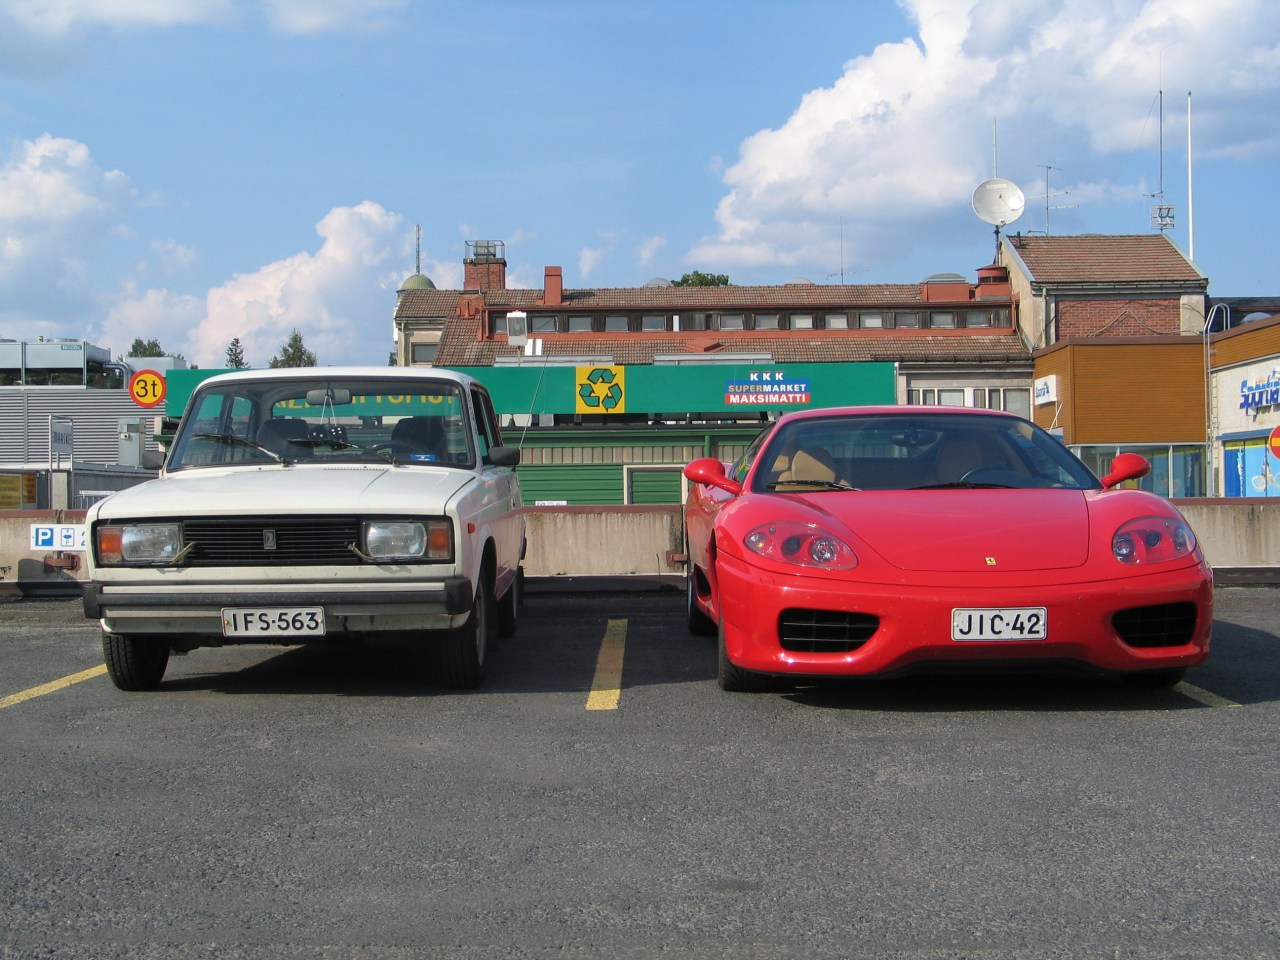
\includegraphics[width=\textwidth]{forside}
\end{figure}

\vfill{}
\begin{description}
\item [{Implementation~code~and~test~results:}]~
\\
\texttt{\url{https://github.com/kasper0406/IO13/tree/master/Project2/}}
\end{description}
\pagebreak{}\tableofcontents{}\pagebreak{}

\section{Introduction}
This report describes the implementation of an external Mergesort and analyses the performance characteristics of the implemented streams and sorting algorithms, as outlined in the project description.


\section{Setup}
This section presents the test setup, how measurements were performed
and gives an overview of the files attached to this report.

\subsection{Test setup}
%!TEX root = rapport.tex
All measurements presented in this report were performed on a computer
with an Intel Core i3-380UM CPU with the following technical
specifications:
\begin{itemize}
\item 2 cores w/HT operating at 1.33GHz
\item 2 x 32KB L1 data cache
\item 2 x 256 KB L2 cache
\item Shared 3MB L3 cache
\end{itemize}
The main memory size of the machine was 1 GB (with approximately 600MB free memory), and the machine was running Ubuntu
Linux 12.04. The hard drive was an USB2 attached Fujitsu MJA2250BH which has the following specifications:

\begin{itemize}
\item 250GB
\item 5,400 RPM
\item 8MB cache
\item 512B sector size
\end{itemize}

The file system had a block size of 4096B and 128kB read ahead.

All implementations have been
written in C++11 and compiled on Linux using the GCC 4.7 compiler. When measurements were performed, the
code was compiled using the \texttt{-O3 -flto -funroll-loops}
optimization flags.

The variations between several runs were insignificant so we choose to run all tests once to be able to run as many configurations as possible.

\subsection{File structure}
The following is a description of the different folders available at
\\
\texttt{\url{https://github.com/kasper0406/IO13/tree/master/Project2/}}
\begin{description}
\item[root] Contains the implementations of the different streams and
  the external heap.

\item[measurements/] Contains the raw measurements used for the plots in the
  report.
\end{description}

\subsubsection{Code structure}
The code has the following source files:
\begin{description}


\item[block.hpp] \texttt{Block} class that represents a node and contains methods for opening streams to the.

\item[buffered\_stream.hpp] Our implementation of a buffered stream.

\item[cached\_stream.hpp] A cached stream that abstracts another stream and provides a cache layer.

\item[CMakeLists.txt] CMake file for the project specifying
  compilation options.

\item[dummy\_stream.hpp] A dummy in-memory stream used for testing.

\item[external\_heap.hpp] Our external heap interface that provides \texttt{insert}, \texttt{extract\_max}, etc.

\item[f\_stream.hpp] Stream implementation using \texttt{fread} and \texttt{fwrite}.

\item[main.cpp] Driver code for calling sanity tests.

\item[mmap\_file\_stream.hpp] Stream implementation using memory mapping and maps the whole file.

\item[mmap\_stream.hpp] Stream implementation using memory mapping and maps block by block.

\item[sys\_stream.hpp] Stream implementation using POSIX \texttt{read} and \texttt{write}.

\item[test.cpp] Driver code for calling test code.

\end{description}

\section{Implementation}
%!TEX root = rapport.tex
This section will present implementation details on how the heap has
been implemented, and how these choices were made. Also the details of
all the implemented streams are discussed.

\subsection{Heap parameters}
\label{sec:implementation:parameters}
\begin{itemize}
  \item $V$ is the maximum number of elements in a node. Hence, a
    node is imperfect if it contains less than $\left\lceil \frac{V}{2}
    \right\rceil$ elements.
  \item $d$ is the fan-out of the tree.
\end{itemize}

\subsection{Heap}
In the paper, the structure of the heap was represented using pointers
such that every node stores pointers to its children and its
parent.

Instead, we chose to embed the structure of the heap
inside an array, such that an array entry contains a reference to a
node in the heap. Then the index of the parent node and the indices of
the child node can be calculated using simple integer operations, and
the corresponding node can be found by looking up in the node array.

% TODO: Lidt bedre forklaring

Using this representation, it is also very easy to swap the position
of two nodes, as the two entries in the array can simply be swapped
(this is required in the insert operation when the last node is
imperfect).

To store the elements of the heap, a big file have been allocated on
disk. This file is (virtually) divided into blocks of size $V$, such
that each block is associated with a node in the tree.

When elements are inserted into the heap, they file may become too
small. Hence when a new block is added, and the file does not have
enough space, the file is extended by $V$ elements. Growing the file
should be handled by the operating system using only constant IOs, and
hence there should be no problem in growing the file every time a new
node is added. As we have enough disk space, we have chosen not to
shrink the file when extracting elements. Again since it should only
require a constant number of IOs we do not believe this will have any
significant influence on our benchmarks.

Every node in the tree has an associated stream, which can read and
write the block associated to the node. Unless mentioned otherwise
in the stream section, the stream for a given node is opened and
closed as it is needed. That is, every time an element should be read
and written, the stream is opened, the operations are executed on the
stream, and then the stream is closed again. This also means that at
most $d + 1$ streams are active at the same time, which happens in
the refill operation.

\begin{figure}
  \centering
  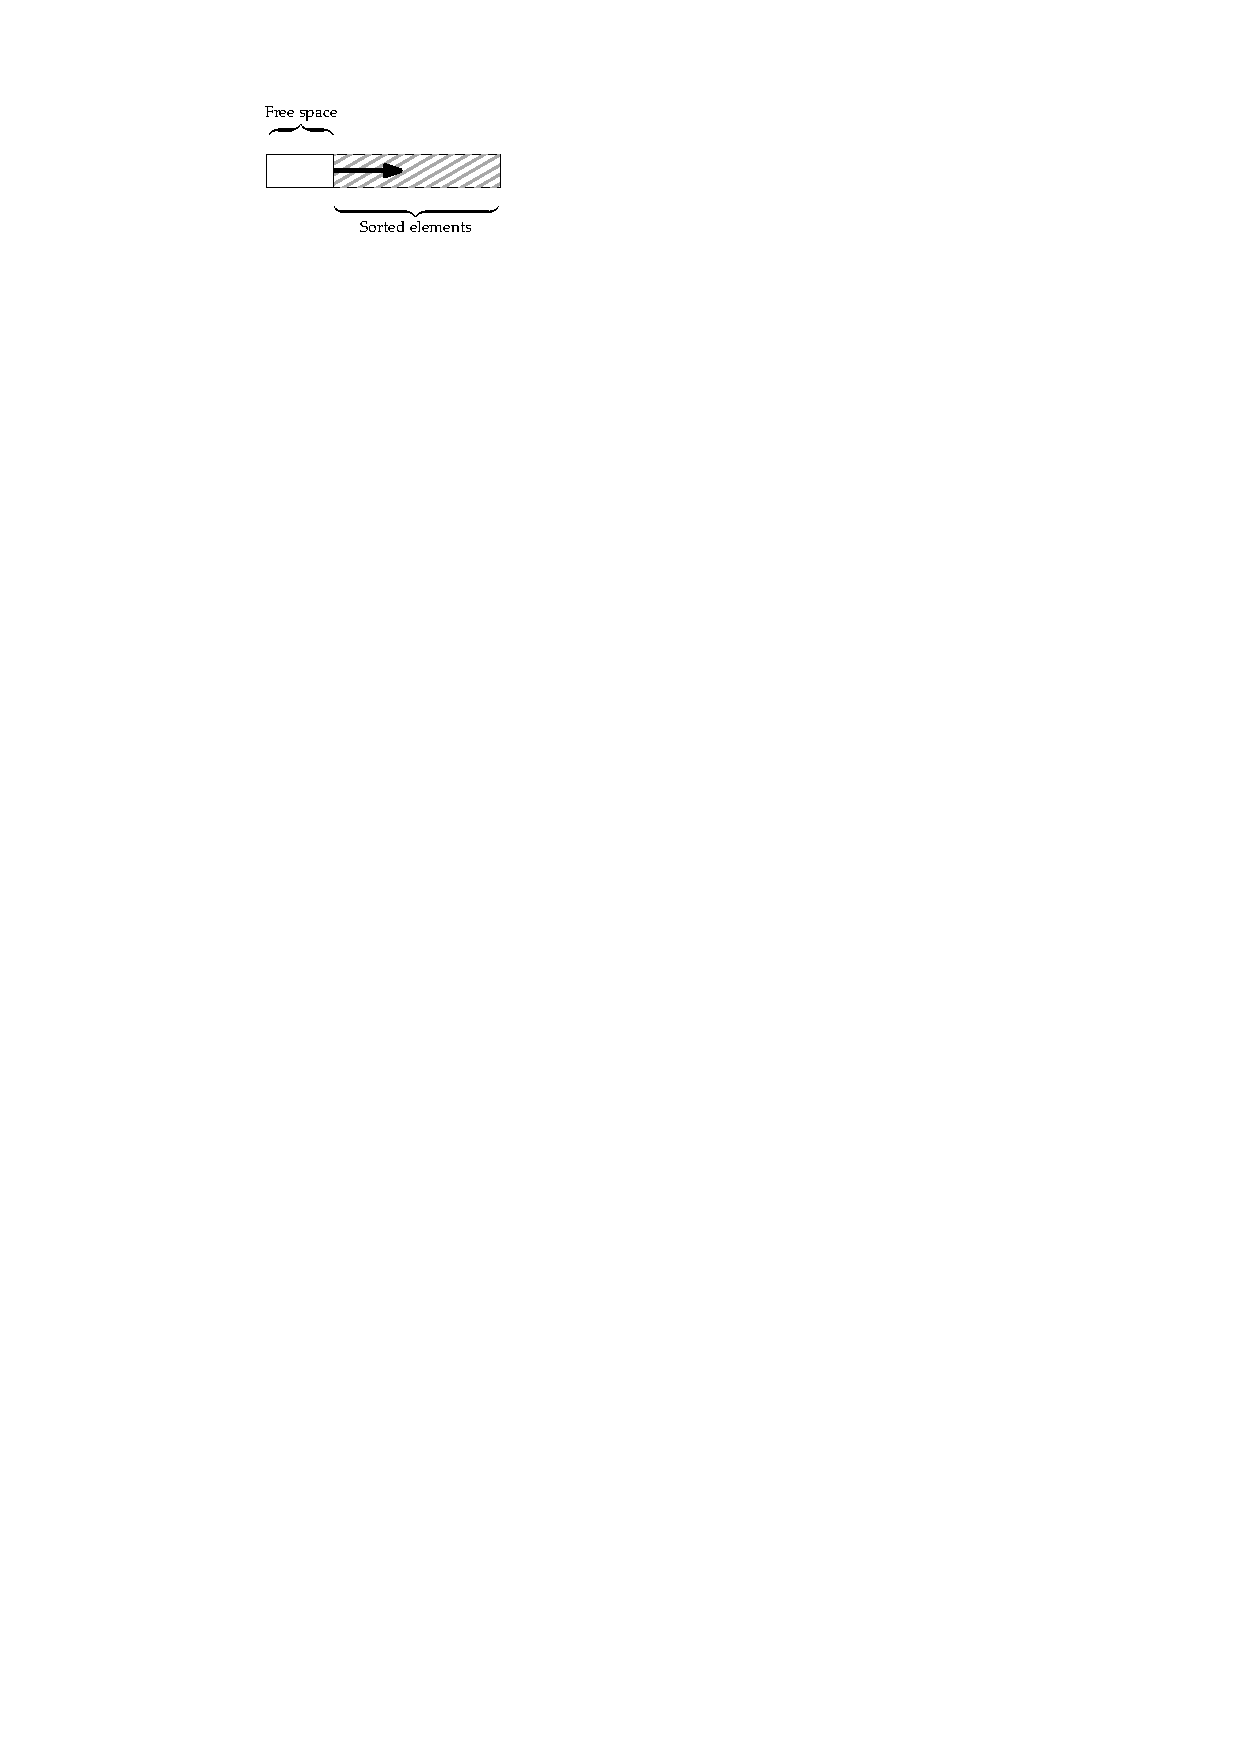
\includegraphics[width=6cm]{node_block}
  \caption{Layout of a block associated with a node. Elements are
    stored in decreasing sorted order, and is placed as far to the
    right as possible.}
  \label{fig:node-block}
\end{figure}

Inside a block, elements are stored to the right in the block in
descending sorted order, as illustrated by
Figure~\ref{fig:node-block}. This layout facilitates forward reading
when extracting the maximum element.

\subsubsection{Sifting}
\label{sec:heap:sifting}
When doing the sift operation, it is required to merge blocks of the
current node and its parent. When doing this, one should be careful
about how many elements are assigned to respectively the parent and
the current node after the merge: If too many elements are transferred
to the parent, such that an element with strictly lower priority is
added to the parent, then the heap invariant between the parent and
its other children may be violated.

On the other hand, it is desired to assign as many elements as
possible to the parent node, as this may delay future refill
operations.

In the paper they assign $\max(r - h, \ceil*{\frac{V}{2}})$ elements to
the child, where $r$ is the sum of the number of elements in the
parent and in the current node, and $h$ is the number of elements
having priority higher than or equal to the parent node. On counter
example to this strategy is when two full blocks are merged, and $h =
0$ (that is, all the child nodes are smaller than the parent node),
then all elements will be assigned to the child, which renders the
parent node imperfect.

We have fixed this by per default to assign
\[
  \max \left( \text{child elements less than minimum in parent}, \ceil*{\frac{V}{2}} \right)
\]
elements to the child. But then it might be the parent gets
overfilled, in which case a sufficient number of the smallest elements
from the parent are transferred to the child node. By construction
this division will satisfy the invariants of the heap.
\\
\\
Two implementations have been made for merging a block:
\begin{description}
\item[Memory inefficient] version where $2V$ elements are buffered,
  and the merging is done in internal memory. This approach has the
  advantage that it only reads forward.
\item[Memory efficient] version where only $V$ elements are
  buffered. The problem with this implementation is to determine how
  many elements should go to the child and to the parent, without
  reading the unbuffered block several times.

  In order to get around this problem, the minimum element in all
  nodes have been cached, which means that the number of elements
  going to the current node (and the parent) can be computed when
  reading the elements of the current node into the buffer. Then the
  elements going to the current node can be written backwards into its
  block, by also reading the buffer and the block of the parent node
  backwards.
\end{description}
We have chosen to investigate both techniques, as we are unsure what
the penalty of reading and writing backwards is, due to read-ahead
etc.. We believe the effect will be different for different types of
streams, as some with large buffers or memory mapped files, may handle
the situation in a better way.

\subsubsection{Verifying correctness}
To ensure the correctness of our heap implementation, the following
three techniques have been used:
\begin{itemize}
\item A graphical representation of the data structure have been
  implemented, enabling us to manually verify small test inputs.
\item A consistency check function has been implemented, which is
  called after every insert and extract operation. The consistency
  check function makes a recursive decent of the nodes in the heap,
  and check that all invariants are satisfied.
\item A sanity test function have been made, where $1\cdot 10^6$
  uniformly random integers was inserted into the heap, and then
  extracted afterwards. It was tested that the integers came out in
  sorted order.
\end{itemize}
All of the above checks passes in our implementation, and we have no
knowledge of bugs.

\subsection{Streams}

To support the heap structure, the stream interface supported the following operations:

\begin{description}
\item[{\texttt{open}}] Opens the stream for read/write
\item[{\texttt{close}}] Closes the stream and deallocates buffers if applicable
\item[{\texttt{peek}}] Peeks at the current location
\item[{\texttt{read\_next}}] Reads at the current location and advances the location
\item[{\texttt{read\_prev}}] Reads at the current location and moves back
\item[{\texttt{write}}] Writes at the current location and advances the location
\item[{\texttt{backward\_write}}] Writes at the current location and moves back
\item[{\texttt{position}}] Return the current location
\item[{\texttt{seek}}] Changes the location
\end{description}

\texttt{read\_prev} and \texttt{backward\_write} were needed for the memory efficient sifting algorithm.

\subsubsection{BufferedStream}

The implementation of buffered stream were slightly more complex than the implementation in project 1 because of the extended stream interface with methods like \texttt{seek} and \texttt{read\_prev}. However, we made a few improvements to make the implementation efficient even with this more general interface. One of the improvements included heuristics to the portion of the file that ends in the buffer. For example, if a requested element that is not in the buffer is at the location right after the buffer ends, then the next portion at the element and onwards is buffered. This improvement could also have been implemented by supplying hints to how the stream is used. Furthermore, a 'write bitmap' were used to determine exactly what needs to be written to disk. This can be important for large buffer sizes.

% TODO: Read map

For the buffered stream, the stream associated with root node was kept open to avoid filling the buffer from disk on each 'extract max' operation.

\subsubsection{MMapStream}

In project 1, the memory mapped stream mapped blocks of the file when they were needed. This is not the most natural way to utilize memory mapped files. Instead, the memory mapped stream used in this projects maps the whole file once and remaps the file if the file size changes. In this way, the operating system is completely in charge of utilizing file caches in the best possible way.

We did test an implementation that worked by mapping blocks when they were needed, but the overhead of remapping made it significantly slower than just mapping the entire file.

\subsubsection{Cached stream}

To make it very fast to retrieve the maximum element of especially the root but also other nodes, a cached stream were implemented. It caches reads but propagates writes to the underlying stream.

The caching is very important for the analysis of the algorithm. If no cache where used in the root node, every extract max operation would result in an I/O. Hence, the algorithm would have the complexity $O(N\log \frac{N}{B})$ instead of $O(\frac{N}{B}\log \frac{N}{B})$. Furthermore, in the refill operation all the children's maximum element is cached at which also would result in additional I/Os.

\subsubsection{Other streams}

A stream (SysStream) using the POSIX methods \texttt{read} and \texttt{write} and a stream (FStream) using \texttt{fread} and \texttt{fwrite} were also implemented. The stream interface almost mapped one-to-one and are therefore not explained in more detail.

The buffer size of \texttt{fread}/\texttt{fwrite} can be found with the constant \texttt{BUFSIZ} in \texttt{<cstdio>}. The buffer size on our system was 4kB.

Similarly to BufferedStream, FStream keeps the stream associated with the root node open.



\section{Benchmarks}
%!TEX root = rapport.tex

\subsection{Sift algorithm variations}
\label{sec:sifting}
As described in Section~\ref{sec:heap:sifting}, two different strategies for sifting have been implemented. A memory efficient using less than $V$ space that reads/writes backwards and a version that uses up to $2V$ space but only reads/writes forwards.

We choose to do a small experiment for our fastest streams with the two sifting implementations, as we were unsure about the penalty (if any) obtained by doing I/O backwards.

For the BufferedStream, the two algorithms were benchmarked for different node sizes and buffer sizes. In all performed experiments, ranging from a buffer size of 4 kB to 256 kB and node size ranging from 2 MB to 8 MB it was found that memory efficient sifting was always superior. We believe this is due to:

\begin{itemize}
\item Buffers and caches, since they are always filled by reading forward.
\item The memory inefficient algorithm interleaves operations on the two streams, where the memory efficient algorithm only uses one stream at a time. For example in the memory inefficient implementation, when the elements of the two nodes are merged into internal memory, elements are read from both of the streams, and even though the streams are buffered, the disk must seek from one part of the disk to another when the buffers needs to be refilled. This is not the case for the memory efficient implementation.
\end{itemize}

For the memory mapped stream, a similar experiment was done. Figure~\ref{fig:m-efficiency} shows the result of this experiment. As can be seen, the memory inefficient algorithm is the fastest for small node sizes, whereas the memory efficient algorithm is faster for large node sizes.

Like before, the stream interleaving done by the memory inefficient algorithm is believed to be contributing to this: For small node sizes it does not matter that much, because relatively few elements are read and most of them can be cached, while for larger node sizes the disk will begin reading from two different areas. To make things worse, the memory inefficient algorithm uses about twice the amount of memory for doing the merge, yielding less space for the operating system to use for caching of the memory mapped file. Therefore, when using a large node size, more pages of the memory mapped file may be swapped to disk, resulting in cache misses later in the test execution.

\begin{figure}
  \centering
  \includegraphics[width=1\columnwidth]{m_efficiency}
  \caption{Comparison of memory inefficient and memory efficient sifting algorithm, when using MMapStream with varying node sizes and 1 GB of elements.}
  \label{fig:m-efficiency}
\end{figure}

\subsection{Parameter weeding}
As described in Section~\ref{sec:implementation:parameters}, the implemented heap has a lot of adjustable parameters which all may have an influence on its performance. In order to limit the time needed for running experiments, the parameter space has been weeded out, such that it does not include obviously bad settings.

We have only considered settings of parameters satisfying the following constraints:
\begin{equation}
  \label{eqn:memory}
  \underbrace{V}_{\textrm{Sifting}} + \underbrace{2P \ceil*{\frac{N}{V}}}_{\textrm{Caching}} + \underbrace{(d + 1)B}_{\mathclap{\substack{
  \textrm{Refill for}\\\textrm{buffered streams}
  }}} \leq M
\end{equation}
\begin{equation}
  \label{eqn:dvn}
  dV\leq N
\end{equation}
Constraint~\ref{eqn:memory} says that all buffers and caches used by the heap should fit into main memory. If this was not the case, memory trashing would occur, resulting in more I/Os than anticipated. Note that for the memory mapped stream there is no explicit buffer, hence when the inequality in \eqref{eqn:memory} is tight, no space is left for the operating system to cache files opened with memory mapping.

Assume a fixed node size, then the performance of sifting improves when the height $h = \log_d{\frac{N}{V}}$ of the tree is decreased because the recursion of sifting ends after fewer iterations. During refilling, $d+1$ streams are open, hence when using a buffered stream $d+1$ buffers are allocated. Therefore, $d$ can be increased as long as the buffers fit into memory.

All configurations not satisfying \eqref{eqn:dvn} will have the same result as $d=\frac{N}{V}$. Moreover parameter values have been increased by a factor of $2$.

\subsection{Streams}
In this section the different streams will be benchmarked and compared.

\subsubsection{Cached stream}
We found that the cached stream improves the performance of the BufferedStream, FStream and SysStream. For SysStream the improvement is expected, since it has no buffer or cache on its own. For the BufferedStream and FStream, a speedup was found with a very small cache size, with decreasing performance when increasing the cache size. We believe this is due to the cache is "conflicting" with the buffers of the underlying streams, but using a very small cache helps when doing the refill operation, since this eliminates the first read from every child node where none or only few elements are are taken.

Figure~\ref{fig:m-cache-size-comparison} shows that MMapStream performs significantly worse when using an extra level of cache. Moreover, the size of the cache does not seem to have a any significant effect on the running time. This is believed to be because that the operating system handles the caching of the memory mapped file itself, and hence adding an extra layer of cache is redundant, and introduces overhead and possibly interferes with the cache strategy employed by the operating system.

\begin{figure}
  \centering
  \includegraphics[width=1\columnwidth]{m_cache_size_comparison}
  \caption{Comparison of the running time for different node sizes using different cache sizes for MMapStream.}
  \label{fig:m-cache-size-comparison}
\end{figure}

In the following experiments, a small cache of 128 elements are used for BufferedStream, FStream and SysStream, whereas no cache is used for MMapStream.

\subsubsection{SysStream and FStream}
By experimenting, we have found that SysStream and FStream performs worse for all tested parameter combinations. Therefore, we have chosen to exclude these streams from all subsequent comparisons.

The reason for the SysStream being slow, is due to its lack of buffering to reduce the number of I/Os. For FStream a buffer is added, however, we found that it was dominated by BufferedStream even with the same buffer size. This is also to be expected, since the buffers used in BufferedStream are optimized for the specific application of an external heap, whereas this is not the case for the more generic FStream.

\subsection{MMapStream}
As seen in figure~\ref{fig:m-efficiency} in section~\ref{sec:sifting}, the node size resulting in the fastest running time for sorting 1 GB of elements is 4 MB. Therefore we have chosen to use this node size when running benchmarks of MMapStream.

From figure~\ref{fig:m:vary-d} it can be seen that a bigger value of $d$ improves running time. Hence, when running benchmarks, we have chosen to make $d$ as large as possible. 

\begin{figure}[h!]
  \centering
  \includegraphics[width=1\columnwidth]{m_d}
  \caption{Running time of MMapStream when varying the $d$ parameter.}
  \label{fig:m:vary-d}
\end{figure}

However, when sorting very big input sizes, the $d$ value can not be increased arbitrary because at least one page from every node should be able to fit the memory mapped file cache, otherwise a lot of trashing would occur. There are two possible solutions to this problem:
\begin{itemize}
\item Increase the node size. This is only possible up to the main memory size, otherwise sifting will begin to put its internal buffer on disk.
\item Restrict $d$ such that there is memory left for the operating system to use as cache when doing refill.
\end{itemize}
Both of the solutions will result in decreased performance, and the latter of the solutions would result in more I/Os, but ultimately this is unavoidable because of the I/O sorting lower bound.

For all the benchmarked input sizes, it has always been possible to simply increase $d$ such that the resulting heap was of height 2.

\subsection{BufferedStream}
\label{sec:bufferedstream}

\begin{figure}[h!]
  \centering
  \includegraphics[width=1\columnwidth]{b_final.pdf}
  \caption{Time for sorting a 1 GB file varying the buffer size (x-axis) and the node size (series)}
  \label{fig:b_final}
\end{figure}

As can be seen in figure~\ref{fig:b_final}, the best performing configuration for buffered stream sorting 1 GB elements is a 32 kB buffer size and a node size of 4 MB. Larger block sizes forces $d$ to be smaller which figure~\ref{fig:m:vary-d} shows hurts performance. But 4 MB node size is also faster than 2 MB node size. We believe this is due to the fact that a larger node size yields more sequential read/write that buffered streams are especially suited for. When the node size increases, the best buffer size also increases. Having a larger buffer size means more sequential reads/writes and higher performance when utilized properly.

Another interesting observation from the figure is that the configurations (except for a node size of 32 MB) begins to perform worse at a point when using larger buffer sizes. This effect is especially visible for a node size of 2 MB. We believe this is due to underutilized buffers. For instance, consider a refill using a node size of 2 MB, $d=512$ and a 32 kB buffer. The algorithm potentially refills $\frac{V}{2}=\frac{\textrm{2 MB}}{2}$ elements and assuming an equal number of elements from each child is moved up, $\frac{V}{2d}=\frac{\textrm{2 MB}}{2 \cdot 512}=\textrm{2 kB}$ elements from each child is used which is significantly less than the buffer size of each child. A similar argument can be used for sifting where a smaller portion is sifted upwards when $d$ is larger and therefore, the buffer is again potentially underutilized.

From this point on, a node size of 4 MB and a buffer size of 32 kB is used when comparing against other other streams.

\subsection{Comparison}

\begin{figure}
  \centering
  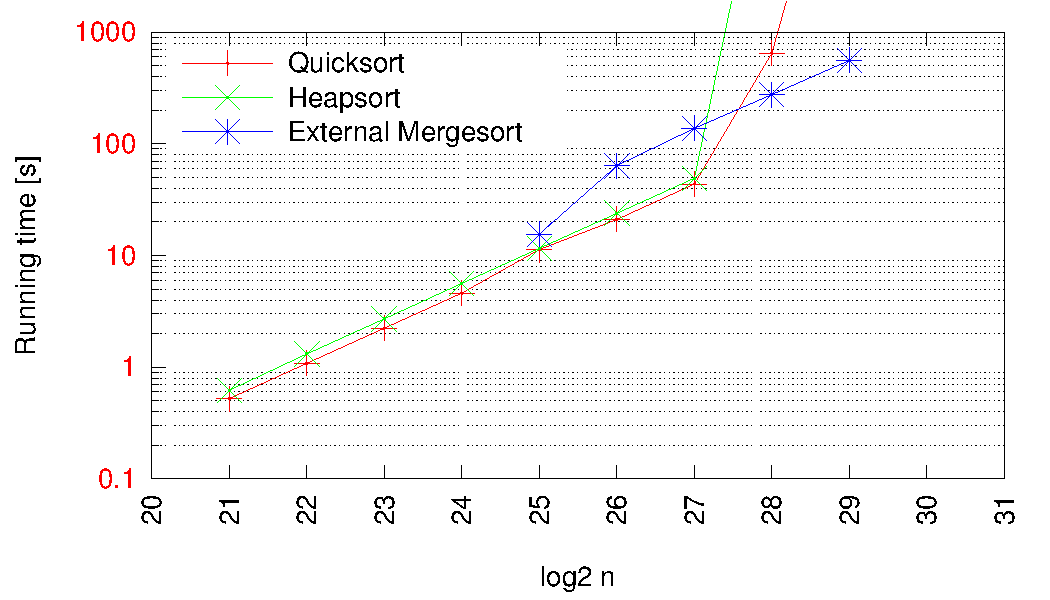
\includegraphics[width=1\columnwidth]{best_sort}
  \caption{Ratio between external mergesort and other sorting algorithms.}
  \label{fig:best_sort}
\end{figure}

We have chosen to omit SysStream and FStream in this comparison because they are inferior to BufferedStream and MMapStream.

Figure~\ref{fig:best_sort} shows how heap sorting using the external heap with BufferedStream and MMapStream compares to external mergesort as implemented in project 1 and in-memory quicksort. It can be seen that the external heapsort is slower than external mergesort with both MMapStream and BufferedStream. This is in agreement with the findings in R. Fadel et. al. \citep{Fadel1999345}.

It seems that the ratio between external heapsort and external mergesort gets worse for larger input sizes. This is not expected since both solutions satisfies the optimal sorting I/O bound. However, note that:
\begin{itemize}
\item In project 1 we saw that the number of input scans in external mergesort was given by the height of the merge tree. For the external heapsort the effect of the tree height is not as profound since the height of the tree does not directly relate to the number of input scans.
\item The number of refill operations is linear in the input size and each refill operation does not only induce a constant number of I/Os when $d$ increases. We may see a more constant ratio if the node size was increased as the input size got larger.
\end{itemize}
Therefore, when an extra level is added to the merge tree, we would expect a drop in the ratio between external mergesort and external heapsort. The reason no drop is seen in the plot is that for the tested input sizes the merge tree always had height 2.

The plot also shows that BufferedStream is approximately 50\% \\ slower than MMapStream. This is opposed to what we found in the external mergesort. We believe this is due to a more random access pattern in the external heapsort which memory mapped files are especially good at due to its least-recently-used cache strategy. It should be noted that the last data point in the series for BufferedStream used a node size of 8 MB instead of 4 MB. It was changed because the measurement with a 4 MB node size showed twice the amount of I/Os than expected. We believe this is due to an underutilized buffer and underutilized read ahead as mentioned in subsection \ref{sec:bufferedstream}.
% TODO: 64 kB buffer as shown as the best configuration of 

\section{Conclusion}
In the course of the project, four different stream implementations
have been made and tested with an eye to the application of external
merge sort. It was possible to single out a winner among the
implemented streams, which was found it to be buffered streams with
2MB of buffer size.

It was found that the implemented external Mergesort tremendously improved the
performance of sorting large input, compared to conventional main
memory sorting algorithms -- for sorting 1GB of integer elements, we
found a performance increase of a factor\todo{insert impressive
  factor. + ~algoritme + ved 2GB var heap/qsort absurd langsomt}.

The overall findings of this project was therefore in agreement with
what should be expected from the I/O-model for analyzing algorithms.
\todo{meget vigtigt med hoejden af traeet (i.e. antallet af I/O)}

\clearpage{}\bibliographystyle{plain}
\addcontentsline{toc}{section}{\refname}\bibliography{ref}

\end{document}
